% mnras_template.tex 
%
% LaTeX template for creating an MNRAS paper
%
% v3.0 released 14 May 2015
% (version numbers match those of mnras.cls)
%
% Copyright (C) Royal Astronomical Society 2015
% Authors:
% Keith T. Smith (Royal Astronomical Society)

% Change log
%
% v3.0 May 2015
%    Renamed to match the new package name
%    Version number matches mnras.cls
%    A few minor tweaks to wording
% v1.0 September 2013
%    Beta testing only - never publicly released
%    First version: a simple (ish) template for creating an MNRAS paper

%%%%%%%%%%%%%%%%%%%%%%%%%%%%%%%%%%%%%%%%%%%%%%%%%%
% Basic setup. Most papers should leave these options alone.
\documentclass[fleqn,usenatbib]{mnras}

% MNRAS is set in Times font. If you don't have this installed (most LaTeX
% installations will be fine) or prefer the old Computer Modern fonts, comment
% out the following line
\usepackage{newtxtext,newtxmath}
% Depending on your LaTeX fonts installation, you might get better results with one of these:
%\usepackage{mathptmx}
%\usepackage{txfonts}

% Use vector fonts, so it zooms properly in on-screen viewing software
% Don't change these lines unless you know what you are doing
\usepackage[T1]{fontenc}
\usepackage{ae,aecompl}


%%%%% AUTHORS - PLACE YOUR OWN PACKAGES HERE %%%%%

% Only include extra packages if you really need them. Common packages are:
\usepackage{graphicx}	% Including figure files
\usepackage{amsmath}	% Advanced maths commands
\usepackage{amssymb}	% Extra maths symbols

%%%%%%%%%%%%%%%%%%%%%%%%%%%%%%%%%%%%%%%%%%%%%%%%%%

%%%%% AUTHORS - PLACE YOUR OWN COMMANDS HERE %%%%%

% Please keep new commands to a minimum, and use \newcommand not \def to avoid
% overwriting existing commands. Example:
%\newcommand{\pcm}{\,cm$^{-2}$}	% per cm-squared

%%%%%%%%%%%%%%%%%%%%%%%%%%%%%%%%%%%%%%%%%%%%%%%%%%

%%%%%%%%%%%%%%%%%%% TITLE PAGE %%%%%%%%%%%%%%%%%%%

% Title of the paper, and the short title which is used in the headers.
% Keep the title short and informative.
\title[Abbie=Smart Person]{The Crystal Ball of Halo Mergers (Not serious title don't worry)}

% The list of authors, and the short list which is used in the headers.
% If you need two or more lines of authors, add an extra line using \newauthor
\author[K. T. Smith et al.]{
Genius 1,$^{1}$\thanks{E-mail: mn@ras.org.uk (KTS)}
Genius 2,$^{2}$
and Genius 3$^{2,3}$
\\
% List of institutions
$^{1}$Royal Astronomical Society, Burlington House, Piccadilly, London W1J 0BQ, UK\\
$^{2}$Department, Institution, Street Address, City Postal Code, Country\\
$^{3}$Another Department, Different Institution, Street Address, City Postal Code, Country
}

% These dates will be filled out by the publisher
\date{Accepted XXX. Received YYY; in original form ZZZ}

% Enter the current year, for the copyright statements etc.
\pubyear{2015}

% Don't change these lines
\begin{document}
\label{firstpage}
\pagerange{\pageref{firstpage}--\pageref{lastpage}}
\maketitle

% Abstract of the paper
\begin{abstract}
I used machine learning to solve the whole universe I'm so smart.
\end{abstract}

% Select between one and six entries from the list of approved keywords.
% Don't make up new ones.
\begin{keywords}
me -- genius -- smart
\end{keywords}

%%%%%%%%%%%%%%%%%%%%%%%%%%%%%%%%%%%%%%%%%%%%%%%%%%

%%%%%%%%%%%%%%%%% BODY OF PAPER %%%%%%%%%%%%%%%%%%

\section{Introduction}

\begin{itemize}
  \item \textit{Broad context: hierarchical merging in LCDM as the primary method of structure formation. We have satellites.}
  According to the standard LCDM model of cosmology, dark matter structures in the universe form hierarchically through series of mergers, eventually growing large enough to host the galaxies and clusters we see today. These larger haloes are thought to form primarily through the accretion of smaller subhaloes. As these subhaloes sink to the center of their host haloes, tidal stripping and dynamical friction cause them to lose mass to their hosts. However, remnants of these subhaloes may survive, and today can be observed by the satellite galaxies that they may come to host.
  \item \textit{Narrower context? The use of N-body simulations as the primary way of studying this, how deterministic interactions are, reliability of cosmological simulations, as discussed in other works?}
  The evolution of dark matter structures is most often studied by running cosmological N-body simulations, where the grouping and merging of haloes can be explicitly tracked. In such simulations, dark matter subhaloes are considered separate objects from their hosts as long as ..... Although these simulations are an excellent tool for studying structure formation in detail, Several models have been created to model how this merging happens. However, many other studies have shown that the fate of a subhalo can be quite stochastic.
  \item \textit{Narrower context: Importance of trying to understand DM populations and what properties of a DM halo drive its evolution. Advantages that could come from having an ML algorithm because it tells us what information is important and if we are/aren't able to predict these sorts of interactions, what that could imply.}
  \item Other works. What do we already know about how these interactions happen? What do we think are the most important properties for determining the outcomes?
  \item In this work: We use a dark matter only simulation and the subhaloes within it, in order to determine the fate (i.e Survival, Mass Loss, Merging Time, Final Position) from its initial conditions at the time of entry.
  \item Motivation for using machine learning. The ability of an ML algorithm to consider all features in an unbiased way. The importance of testing models with a lot of features so that we can say whether the information is really there or not.
    \item The Nadler et al paper. Machine learning as shown to be a promising tool for astronomy and these types of interactions in particular.
  \item Paragraph that says what all of the sections are. In Section 2, we describe the simulation and data that was used, as well as the methods to properly reduce the data into the desired sample. In section 3, we cover the machine learning methods used and any special techniques applied to each predictor. In Section 4, we share the results of the predictions for each of the measures of fate and a simpler form?? (equation?? if we can) that can be used to predict each of the fates. Finally, in Section 5 we discuss implications of the results for both observation and theory.
\end{itemize}

This is how you'd have a little code-text thing: \texttt{mnras\_sample.tex}.
And this is how I'd cite stuff when I finally read some papers: \citet{Others2013}, \citep[e.g.][]{Author2012}.

\section{Simulation/Description Of Data}
	Our analysis makes use of VISHNU, a cosmological N-body simulation with 1000 snapshots. VISHNU contains 1680\textsuperscript{3} particles in a volume of 130h\textsuperscript{-1} cMpc and uses WMAP-1 cosmology (\citet{Springel2013}; $\Omega$\textsubscript{m} = 0.25, $\Omega$\textsubscript{$\Lambda$} = 0.75, $\Omega$\textsubscript{b} = 0.04, $\sigma$\textsubscript{8} = 0.8, \textit{n\textsubscript{s}} = 1.0, \textit{h} = 0.7). Each dark matter particle has mass \textit{m\textsubscript{p}} = 3.215 $\times$ 10\textsuperscript{7}h\textsuperscript{-1} M\textsubscript{\(\odot\)}, and subhalos can contain as few as 2 particles. The ROCKSTAR halo finder was used to identify halos and subhalos, and merger trees were constructed with Consistent-Trees (\citet{Behroozi2013b}).
\par
    From the merger trees, we select subhalos of the most massive progenitors of host halos at \textit{z}=0. These subhalos are allowed to have further substructure inside of them but cannot, at any point during their infall, become sub-substructure themselves. To help mitigate resolution uncertainties, we select only subhalos which consist of 1000 particles (total mass 3.215 $\times$ 10\textsuperscript{10}h\textsuperscript{-1} M\textsubscript{\(\odot\)}) or more at their time of accretion. We define the accretion point of a subhalo as the last timestep before a subhalo enters its host. As such, at the initial time of accretion, the will-be subhalos are still host halos themselves. Once the subhalo has entered its host, however, it cannot leave again (so, a flyby interaction would not be considered on its first pass but will be considered on a later pass if it falls back into and remains inside the host). Once it has been accreted, the subhalo must have one of two fates: merge with the host, or remain a bound, identified subhalo within that host until today. Following uncertainties in subhalo mass loss shown by \citet{VDB2018}, once a subhalo has lost more than 90\% of its mass, it is considered to be merged.
\par
    In addition to making cuts for resolution, some merging interactions were removed due to their unphysical behavior, likely as a result of errors in the merger trees. \textbf{INSERT NUMBER} Subhalos were removed that gained more than 10 times their mass (\textit{or some threshold.. I don't know yet what's best yet}) during infall. These subhalos likely had their identifications changed as they moved close to the center of the host. \textbf{INSERT NUMBER} subhalos were removed because their initial mass was larger than that of its supposed host. \textbf{INSERT NUMBER} subhalos were removed because their positions were outside of their host's virial radius after periodic boundary conditions were corrected for. \textbf{INSERT NUMBER} subhalos were removed because their time of merging was earlier than their time of entry?? \textit{Show a few cases of these strange orbits/mass loss histories??}
\par
	Although we have attempted to correct for these errors, there remains the possibility that erroneous cases still exist within our sample. We have made a hard cut to remove halos that gain mass, but there may be still be cases where an identification of a halo was changed within our sample. Possible other cases we found: Weird looking orbits that weren't in initial filtering. Some discussion of the cases that could possibly still exist in the data due to difficulty in being able to filter them out/ find a general way to search for them? \textit{Something that gives some estimation of how many cases might be like this? To ensure that it's not some large part of the sample and the reason we can't predict things. Mention that we removed about 2\% of the total number so even if you assume the same portion is wrong it shouldn't be the source of the stochasticity?}
\par
    Our resulting sample includes a total of \textbf{INSERT NUMBER} subhalo-halo interactions. Distributions of this sample with respect to host masses, mass ratios, and the scale factor of the time of entry are shown in Fig.~\ref{fig:combined_distributions_logBin}. The most common interactions in our sample are mergers of lower mass ratio that occurred more recently. However, our sample also spans the space of more equal mass and higher redshift mergers, with hundreds of interactions shown in many of the bins in Fig.~\ref{fig:combined_distributions_logBin}. \textit{Some reference to how many of these are expected? Indication that this is a representative sample of what we expect to see slash agreement with other simulations?}
\par
    For both the host halo and subhalo at the timestep of infall, and at either the timestep right before merging or at z=0, we take several physically-motivated parameters to describe the interaction between the halos. Table 1 lists these parameters and includes a brief description of each. \textit{Include ALL parameters that we took and then somehow mark the ones that we kept or only mention the ones that we kept. I don't want a table of a billion things but also don't want any question that we didn't cover everything}. From the parameters taken from the merger trees, we calculated some additional parameters. These include the eccentricity, mass ratio (M\textsubscript{ratio}=M\textsubscript{sub}/M\textsubscript{host}), relative distances and relative velocities? \textit{How much to go over these, or do we even need to mention calculating stuff like relative distance because it's so obvious.}
\par
    As preparation for using machine learning, we split the data into train and test sets, with 80\% of the data to be used for training and 20\% to be used for testing. These subsamples are selected randomly from the total sample. \textit{Counts and some simple statistics of these sets are shown in Table 2. Averages and standard deviations of these samples are similar, showing that the test set is representative of the training set.} The data was also scaled and normalized to have a mean of zero and unit variance. For training the machine learning models, the training set was further divided into training and validation sets, also using an 80/20 split. From the original dataset, this means the data was split as 64\% training, 16\% validation, and 20\% testing.


\begin{figure*}
	% To include a figure from a file named example.*
	% Allowable file formats are eps or ps if compiling using latex
	% or pdf, png, jpg if compiling using pdflatex
	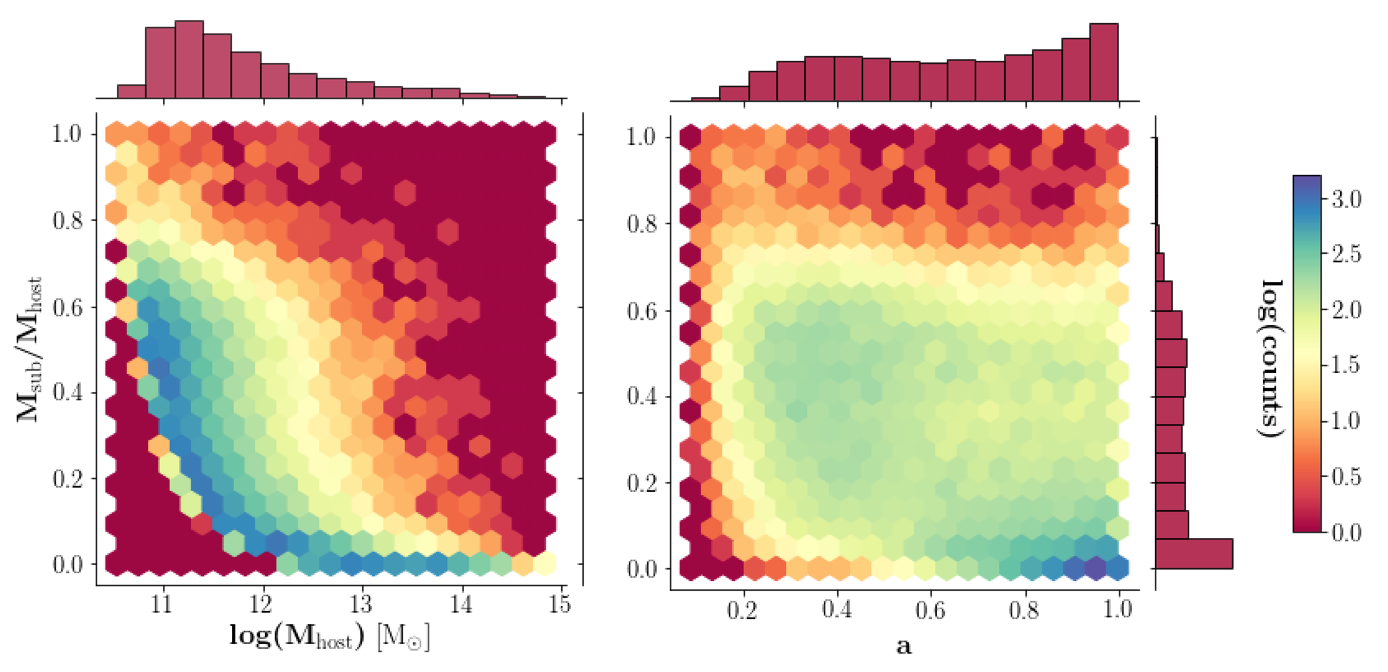
\includegraphics[width=\textwidth]{Figures/combined_distributions_logBin}
    \caption{Distributions of the merging interactions within our sample, in two different two-dimensional spaces. The left panel shows the distribution of mergers in the space of the host mass (x-axis) and the mass ratio (y-axis) of the interaction. The right panel shows the distribution of mergers in the space of the scale of initial entry of the subhalo (x-axis) and again, the mass ratio of the interaction on the y-axis. Within each hexagonal bin, the counts of interactions are shown, on a logarithm scale, by the colorbar. Histograms show the one-dimensional distribution of host masses (above the left panel), scale of entry (above the right panel) and mass ratios to the right of the right panel). Most interactions occur at lower mass ratios and for smaller host halos, but the spaces are still well-spanned over a range of interactions in both panels. }
    \label{fig:combined_distributions_logBin}
\end{figure*}

\section{Machine Learning Methods}
Discussion and description of the various machine learning models that were used. Might also contain subsections? For data, for each method, for feature selection? Or for each type of method? The second way is how I did it here but it`s definitely not necessarily the best way. 


\subsection{Random Forests}
\label{sec:rf} % used for referring to this section from elsewhere
\begin{itemize}
	\item Basic description of the algorithm and how it works.
    \item Advantages and disadvantages.
    \item regression vs classification?
\end{itemize}

\subsection{Gradient Boosting Regressors}
\label{sec:gbr} % used for referring to this section from elsewhere
\begin{itemize}
	\item Basic description of the algorithm and how it works.
    \item Advantages and disadvantages.
    \item regression vs classification?
\end{itemize}

\subsection{Neural Networks}
\label{sec:nn} % used for referring to this section from elsewhere
\begin{itemize}
	\item Basic description of the algorithm and how it works.
    \item Advantages and disadvantages.
    \item regression vs classification?
\end{itemize}

\subsection{Feature Selection}
\label{sec:feature selection} % used for referring to this section from elsewhere
\begin{itemize}
    \item Initially, our sample contained \textbf{INSERT NUMBER} parameters (or features) to describe each interaction. Reducing the dimensionality of the data? Checks for important and unimportant parameters. How we are sure that the number of features we gave the model is correct and optimal, how were we able to get rid of some of the unimportant parameters. 
    \item Description of the different methods we used to check for dimensionality reduction?
    \item According to selected features, what do the best spaces look like for some of the things we want to predict? Shown for survival and mass loss in \ref{fig:bestSpaces_vartree}.
\end{itemize}
    % Best-spaces figure
\begin{figure*}
	% To include a figure from a file named example.*
	% Allowable file formats are eps or ps if compiling using latex
	% or pdf, png, jpg if compiling using pdflatex
	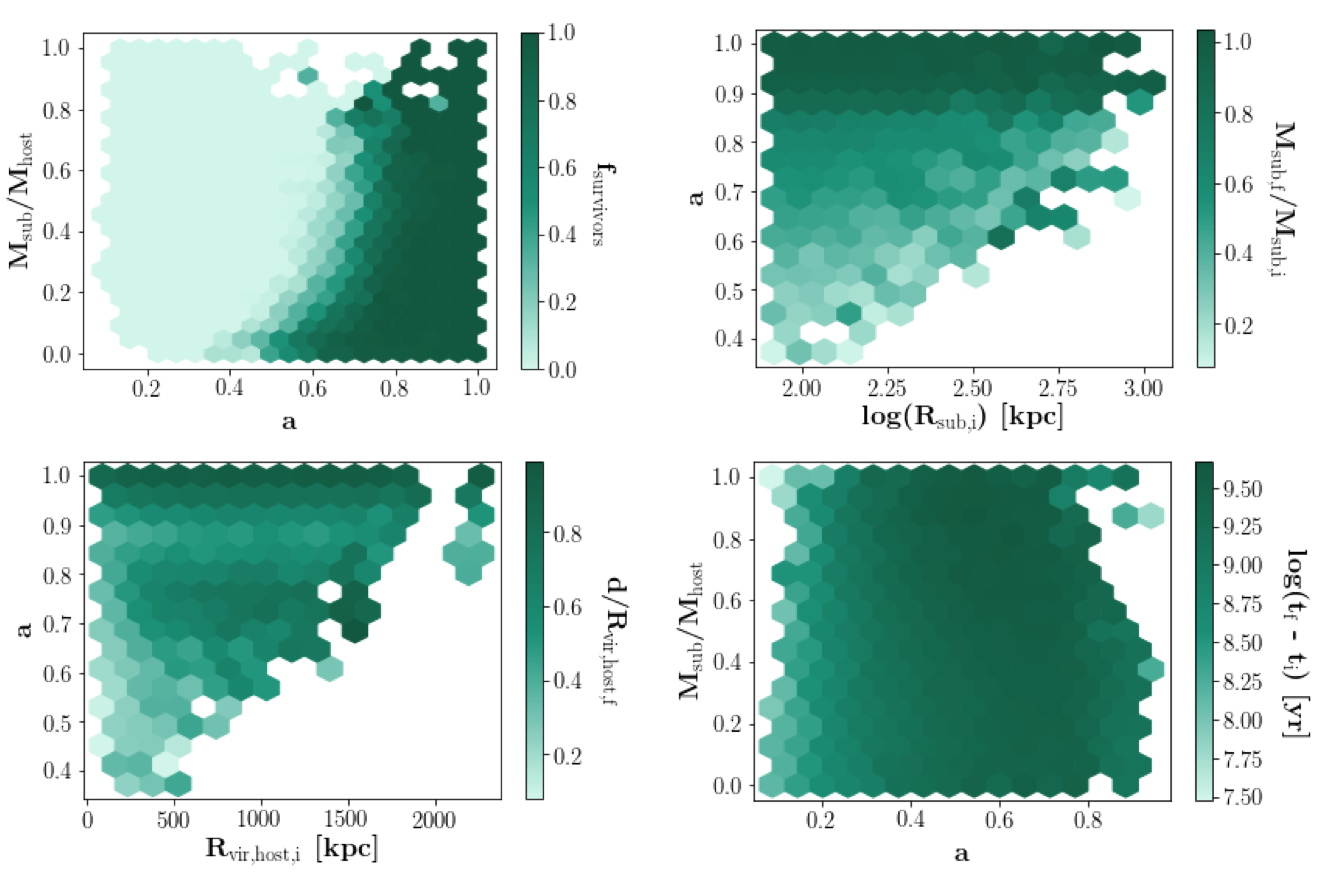
\includegraphics[width=\textwidth]{Figures/bestSpaces_vartree}
    \caption{Distributions of the predicted quantity of interest with respect to the two parameters that are most responsible for its variations. In each panel, the parameter that causes the most variation is shown on the x-axis, and the parameter that causes the second most variation is shown on the y-axis. In addition, in each panel the colorbar shows the average values of the quantity of interest within a bin. The top left panel shows the fraction of surviving subhalos. The top right panel shows the fraction of subhalo mass that remains for surviving subhalos. The bottom left panel shows the fractional distance of surviving subhalos from their host's center. The bottom right panel shows the elapsed time for a subhalo to merge. In each instance, some pattern of color striation can be seen to represent the importance of the two parameters shown. However, it is clear that the survival of a subhalo is by far the most drastically divided and well-defined by this two-dimensional space. }
    \label{fig:bestSpaces_vartree}
\end{figure*}

?? Discussion of any other models tried that didn't perform as well? Mention that other models were tested or don't mention at all? Talk at all about getting equations from (simpler) models if we wanted to include both? Survival has a straightforward equation that does pretty well, although a non-equation model does better. All of the regression models have no simple solution. Is it worth mentioning/presenting the simple solution?

\section{Results}
This section will probably be split into subsections, such as Section~\ref{sec:survival} below.

\subsection{Survival}
\label{sec:survival} % used for referring to this section from elsewhere

For the entire sample of subhaloes, we first try to predict whether or not a halo will survive until today (1) or merge particles with the host (0) during its infall.
\begin{itemize}
		\item The best method: Show the results of whatever machine learning algorithm worked the BEST. Plots of adding parameters for different tolerances (on the validation set) and explain choices for the fiducial confidence.
	\item The parameters: the best combination of parameters, other combinations that were found to be good, too. Whether or not those agree with feature selection methods that we used. Present the best order of the parameters, and show how much information is gained by adding each parameter and how it levels off. Explain how we have decided to reduce the full set of data to the smallest subset of parameters.
    \item With the chosen fiducial tolerance and subset of parameters, show how well the model performs on the test set and report a final accuracy.
    \item A predictive equation?? Show the logistic regression results and the equation that it produces? I can't remember how well it worked. Not sure if it's even worth mentioning.
\end{itemize}

\begin{figure*}
	% To include a figure from a file named example.*
	% Allowable file formats are eps or ps if compiling using latex
	% or pdf, png, jpg if compiling using pdflatex
	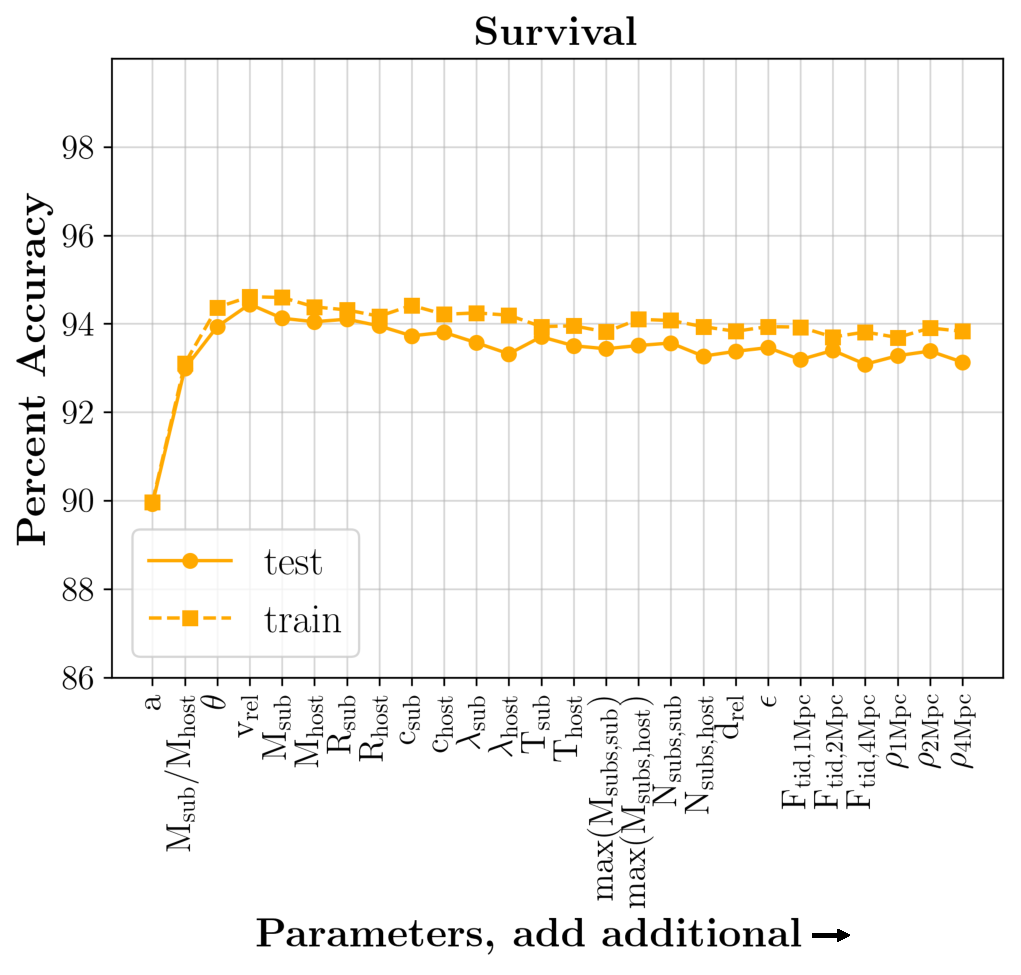
\includegraphics[width=\columnwidth]{Figures/survival_predictions}
    \caption{Survival.}
    \label{fig:survival_predictions}
\end{figure*}

\begin{figure*}
	% To include a figure from a file named example.*
	% Allowable file formats are eps or ps if compiling using latex
	% or pdf, png, jpg if compiling using pdflatex
	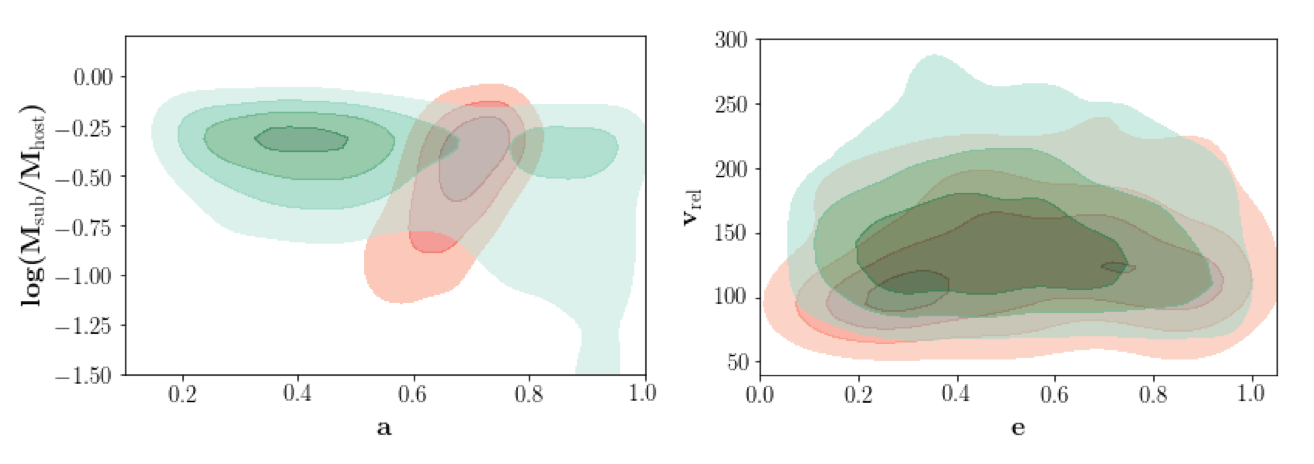
\includegraphics[width=\textwidth]{Figures/survival_contours}
    \caption{Mass loss contours.}
    \label{fig:survival_contours}
\end{figure*}

\subsection{Mass Loss}
\label{sec:mass loss}
\begin{itemize}
	\item The best method: Show the results of whatever machine learning algorithm worked the BEST. Plots of adding parameters for different tolerances (on the validation set) and explain choices for the fiducial confidence.
	\item The parameters: the best combination of parameters, other combinations that were found to be good, too. Whether or not those agree with feature selection methods that we used. Present the best order of the parameters, and show how much information is gained by adding each parameter and how it levels off. Explain how we have decided to reduce the full set of data to the smallest subset of parameters.
    \item With the chosen fiducial tolerance and subset of parameters, show how well the model performs on the test set and report a final accuracy.
\end{itemize}

\begin{figure*}
	% To include a figure from a file named example.*
	% Allowable file formats are eps or ps if compiling using latex
	% or pdf, png, jpg if compiling using pdflatex
	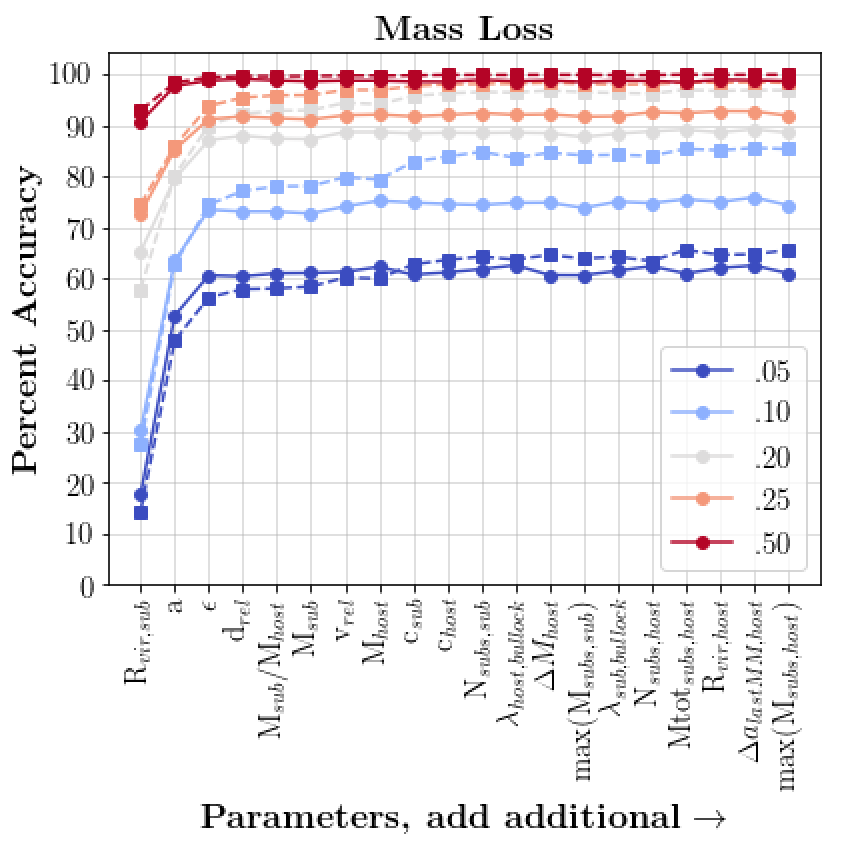
\includegraphics[width=\columnwidth]{Figures/massloss_predictions}
    \caption{Mass loss.}
    \label{fig:massloss_predictions}
\end{figure*}

\begin{figure*}
	% To include a figure from a file named example.*
	% Allowable file formats are eps or ps if compiling using latex
	% or pdf, png, jpg if compiling using pdflatex
	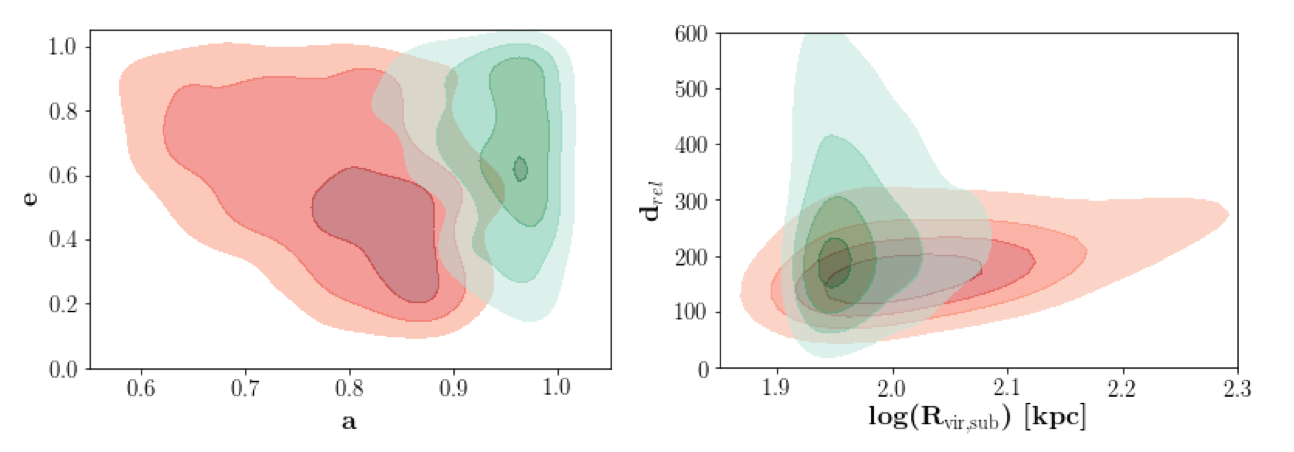
\includegraphics[width=\textwidth]{Figures/massloss_contours}
    \caption{Mass loss contours.}
    \label{fig:massloss_contours}
\end{figure*}

\begin{figure*}
	% To include a figure from a file named example.*
	% Allowable file formats are eps or ps if compiling using latex
	% or pdf, png, jpg if compiling using pdflatex
	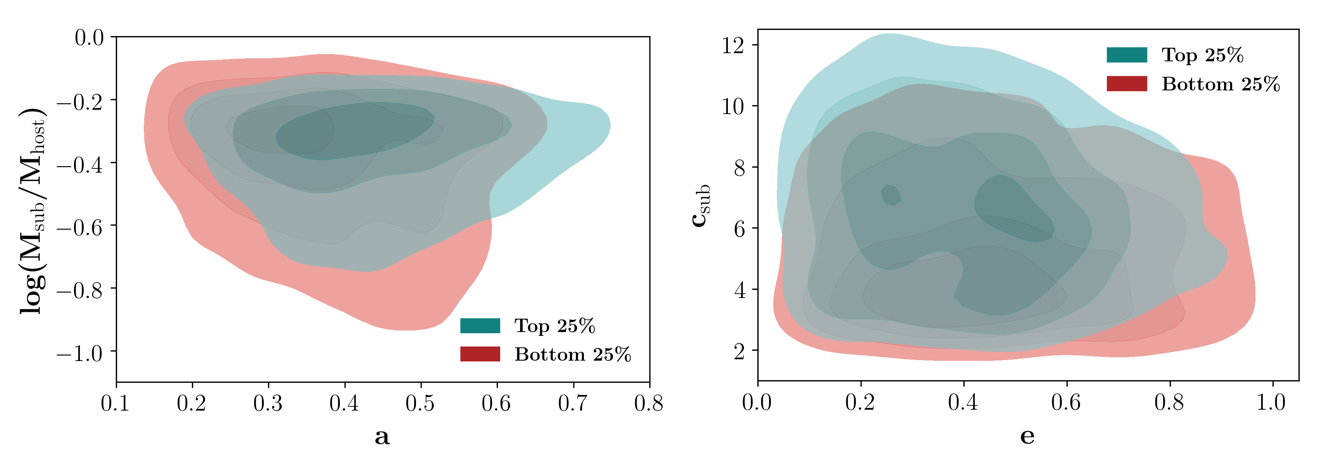
\includegraphics[width=\textwidth]{Figures/time_contours}
    \caption{Time contours.}
    \label{fig:time_contours}
\end{figure*}

\subsection{Final Position}
\label{sec:position}
\begin{itemize}
	\item The best method: Show the results of whatever machine learning algorithm worked the BEST. Plots of adding parameters for different tolerances (on the validation set) and explain choices for the fiducial confidence.
    \item The parameters: the best combination of parameters, other combinations that were found to be good, too. Whether or not those agree with feature selection methods that we used. Present the best order of the parameters, and show how much information is gained by adding each parameter and how it levels off. Explain how we have decided to reduce the full set of data to the smallest subset of parameters.
    \item With the chosen fiducial tolerance and subset of parameters, show how well the model performs on the test set and report a final accuracy.
\end{itemize}

\begin{figure*}
	% To include a figure from a file named example.*
	% Allowable file formats are eps or ps if compiling using latex
	% or pdf, png, jpg if compiling using pdflatex
	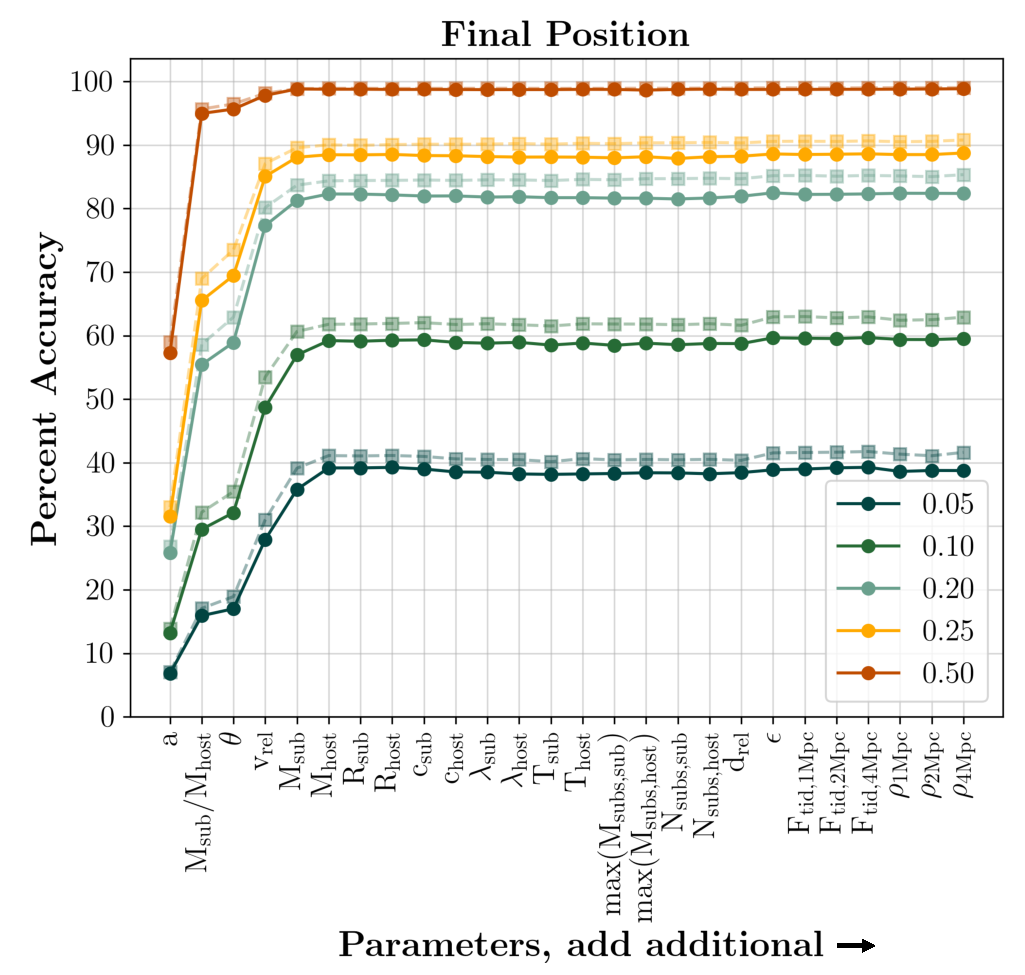
\includegraphics[width=\columnwidth]{Figures/position_predictions}
    \caption{Position.}
    \label{fig:position_predictions}
\end{figure*}

\begin{figure*}
	% To include a figure from a file named example.*
	% Allowable file formats are eps or ps if compiling using latex
	% or pdf, png, jpg if compiling using pdflatex
	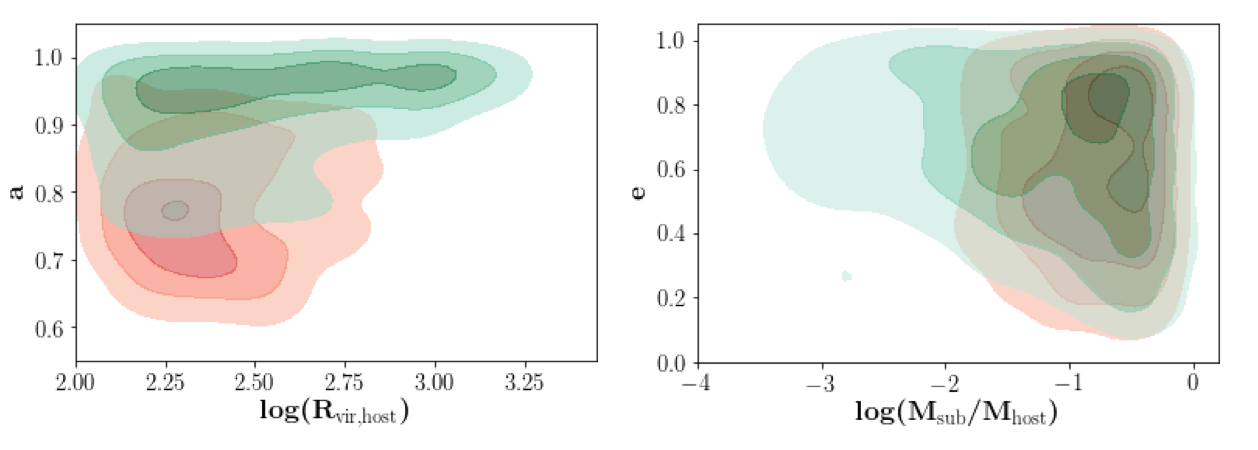
\includegraphics[width=\textwidth]{Figures/position_contours}
    \caption{Position contours.}
    \label{fig:position_contours}
\end{figure*}

\subsection{Merge Time}
\label{sec:merge time}
\begin{itemize}
	\item The best method: Show the results of whatever machine learning algorithm worked the BEST. Plots of adding parameters for different tolerances (on the validation set) and explain choices for the fiducial confidence.
	\item The parameters: the best combination of parameters, other combinations that were found to be good, too. Whether or not those agree with feature selection methods that we used. Present the best order of the parameters, and show how much information is gained by adding each parameter and how it levels off. Explain how we have decided to reduce the full set of data to the smallest subset of parameters.
    \item With the chosen fiducial tolerance and subset of parameters, show how well the model performs on the test set and report a final accuracy.
\end{itemize}

\begin{figure*}
	% To include a figure from a file named example.*
	% Allowable file formats are eps or ps if compiling using latex
	% or pdf, png, jpg if compiling using pdflatex
	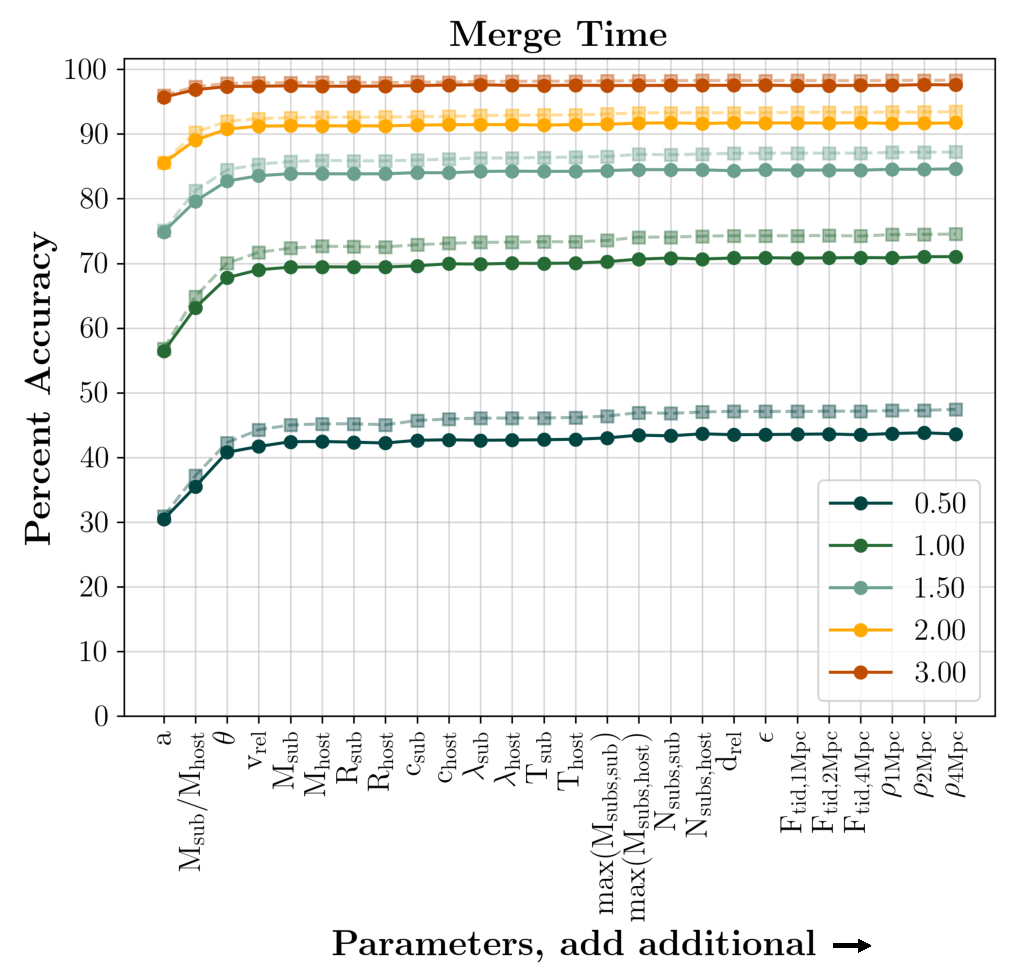
\includegraphics[width=\columnwidth]{Figures/time_predictions}
    \caption{Merge Time.}
    \label{fig:time_predictions}
\end{figure*}

\subsection{Access to the Results?}
Do we want to have there be some way to access the black box/trained model if we can't get an analytical form of the predictions? Do people include parts in their paper about where to find their code or anything? Do people need to be able to find my code somewhere?

\subsection{Some Useful LATEX Stuff - Not part of paper}
Just some stuff that came with the template that I'll probably need to reference at some point when I have to add Figures and equations and all that to the above sections.

This is how I would enter math or an equation e.g. $2\times3=6$
or $v=220$\,km\,s$^{-1}$. A numbered equation:

\begin{equation}
    x=\frac{-b\pm\sqrt{b^2-4ac}}{2a}.
	\label{eq:quadratic}
\end{equation}
Refer to as equation~(\ref{eq:quadratic}).

Refer to figures as e.g. Fig.~\ref{fig:example_figure}, and tables as
e.g. Table~\ref{tab:example_table}.

% Example table
\begin{table}
	\centering
	\caption{Caption for the table.}
	\label{tab:example_table}
	\begin{tabular}{lccr} % four columns, alignment for each
		\hline
		A & B & C & D\\
		\hline
		1 & 2 & 3 & 4\\
		2 & 4 & 6 & 8\\
		3 & 5 & 7 & 9\\
		\hline
	\end{tabular}
\end{table}

\section{Discussion}
\begin{itemize}
	\item Discuss the parameters that were chosen to be important. Are they the same across all outcomes, are they what we expect them to be. Discussion of any that might be surprising/some physically motivated speculation as to why those chosen make or don't make sense.
    \item What went wrong for the outcomes that can't be predicted very well. Show/Discuss specific cases where outcomes are predicted well/not well. Is there a fundamental difference in the distribution between good/bad predictions in any parameter space? Is there anything common amongst the halos that are predicted poorly for different parameters (are the same haloes predicted poorly across multiple outcomes)
    \item Possible missing parameters. Anything else that might contribute to the predictions that we haven't included. What do the distributions in parameter space tell us about the ML failing to capture information vs the outcomes having some inherent randomness.
    \item Robustness of the machine learning results. Investigation of data size to show that we weren't constrained by amount of data. Cost curves during training? ROC curves? Is it possible the model could have done better given a different tuning/training of the ML algorithms? Discussion of possible underfitting/overfitting of the models. Room for improvement in the ML methodology.
    \item Possible uses/implications of the models for simulation. Is this usable to make predictions for any of the outcomes? If it's not, what does that tell us about the nature of these simulations.
    \item Possible use/implications for observation. Is there anything we can say about distributions that we can expect around the MW or other galaxies. Discussion of future works related to this?

\end{itemize}


\section{Conclusions}

\begin{itemize}
	\item Restate the predictions, how well to the fiducial confidence can do for each of the outcomes. Restate what the most important features are and the smallest subset of features for each outcome needed to do a good job.
	\item Implications for theory. Usability of an equation (if one is able to be made). Looking further/future work into looking at the actual orbits or figuring out what's up with the failed cases.
\end{itemize}

\section*{Acknowledgements}

I would like to thank the academy, ...

%%%%%%%%%%%%%%%%%%%%%%%%%%%%%%%%%%%%%%%%%%%%%%%%%%

%%%%%%%%%%%%%%%%%%%% REFERENCES %%%%%%%%%%%%%%%%%%

% The best way to enter references is to use BibTeX:

%\bibliographystyle{mnras}
%\bibliography{example} % if your bibtex file is called example.bib


% Alternatively you could enter them by hand, like this:
% This method is tedious and prone to error if you have lots of references
\begin{thebibliography}{99}
\bibitem[\protect\citeauthoryear{Author}{2012}]{Author2012}
Author A.~N., 2013, Journal of Improbable Astronomy, 1, 1
\bibitem[\protect\citeauthoryear{Others}{2013}]{Others2013}
Others S., 2012, Journal of Interesting Stuff, 17, 198
\bibitem[\protect\citeauthoryear{Springel}{2013}]{Springel2013}
Springel A.~N., OtherStuff NotReal. 2013, Journal of Improbable Astronomy, 1, 1
\bibitem[\protect\citeauthoryear{Behroozi}{2013}]{Behroozi2013b}
Behroozi A.~N., OtherStuff NotReal. 2013, Journal of Improbable Astronomy, 1, 1
\bibitem[\protect\citeauthoryear{van den Bosch}{2018}]{VDB2018}
van den Bosch A.~N., OtherStuff NotReal. 2018, Journal of Improbable Astronomy, 1, 1
\end{thebibliography}

%%%%%%%%%%%%%%%%%%%%%%%%%%%%%%%%%%%%%%%%%%%%%%%%%%

%%%%%%%%%%%%%%%%% APPENDICES %%%%%%%%%%%%%%%%%%%%%

\appendix

\section{Some extra material}

If I wanted to present additional material which would interrupt the flow of the main paper, that would go here.

%%%%%%%%%%%%%%%%%%%%%%%%%%%%%%%%%%%%%%%%%%%%%%%%%%


% Don't change these lines
\bsp	% typesetting comment
\label{lastpage}
\end{document}

% End of mnras_template.tex